\newcolumntype{x}[1]{>{\centering\arraybackslash\hspace{0pt}}p{#1}}
\newcolumntype{M}[1]{>{\centering\arraybackslash\hspace{0pt}}m{#1}}
%\definecolor{myBlue}{RGB}{210, 230, 255}
\definecolor{myBlue}{RGB}{217, 230, 242}

En aquest capítol es detallen els experiments realitzats i els resultats obtinguts a partir d'aquests.

\section{Experiments realitzats}
	Podeu trobar el codi dels scripts realitzats a l'anex del treball.
	\subsection{Comparació detectors de keypoints}
		Tot i que la velocitat d'execució no és un factor determinant pel projecte, s'ha realitzat una comparació inicial de la velocitat d'execució dels algorismes de detecció de keypoints.\\\\
		Es comparen els següents algorismes:
		\begin{itemize}
			\item{Harris}
			\item{SIFT}
			\item{SURF}
			\item{ORB}
			\item{MSER}
		\end{itemize}
		Per mesurar el temps d'execució, s'agafa la mitja de 5 execucions de la funció d'obtenció de keypoints utilitzada.
	\subsection{Comparació detecció i extracció de keypoints}
		En aquest experiment s'analitzen els diversos algorismes de detecció i extracció de keypoints, tant en la velocitat d'execució com en fiabilitat, que serà el més important pel sistema desenvolupat.\\\\
		Es compararan els següents algorismes:
		\begin{itemize}
			\item{Harris + SIFT}
			\item{Harris + LATCH}
			\item{SIFT + SIFT}
			\item{SIFT + LATCH}
			\item{ORB + ORB}
			\item{ORB + BRISK}
			\item{MSER + SURF}
			\item{MSER + DAISY}
		\end{itemize}
\newpage
\section{Resultats i comparació d'algorismes}
	\subsection{Detectors de keypoints}
	En primer lloc s'han realitzat proves amb imatges típiques de visió per computador.
		\begin{figure}[!htb]
			\minipage{0.32\textwidth}
				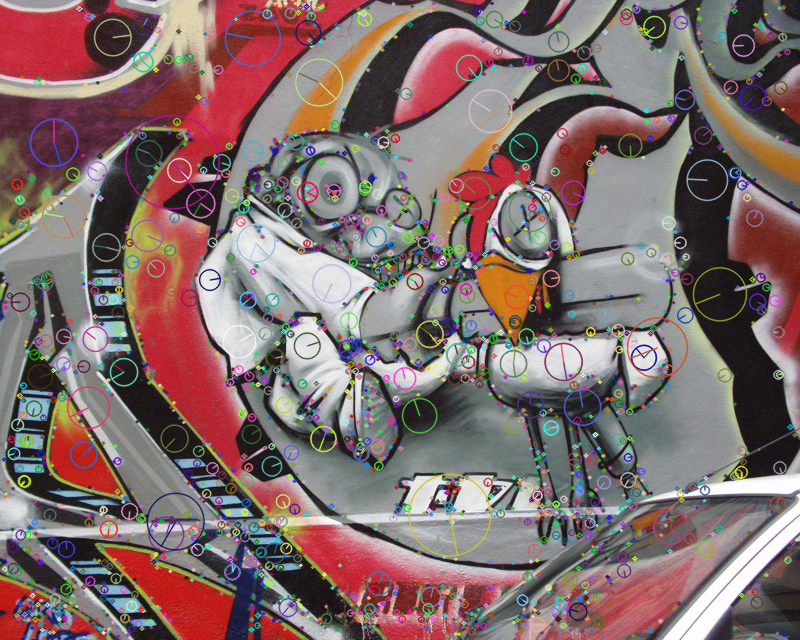
\includegraphics[width=\linewidth]{images/RobotKp}
				\label{fig:awesome_image1}
			\endminipage\hfill
			\minipage{0.32\textwidth}
				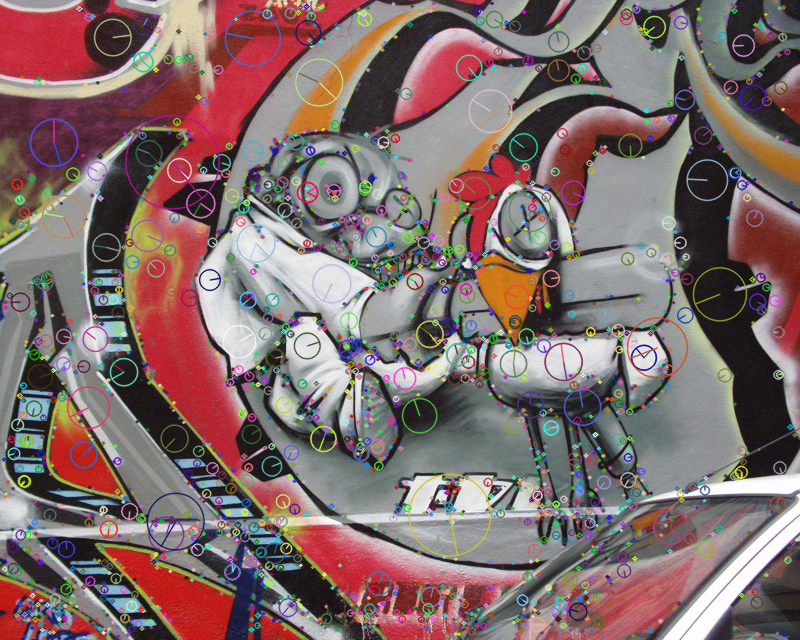
\includegraphics[width=\linewidth]{images/RobotKp}
				\label{fig:awesome_image2}
			\endminipage\hfill
			\minipage{0.32\textwidth}%
				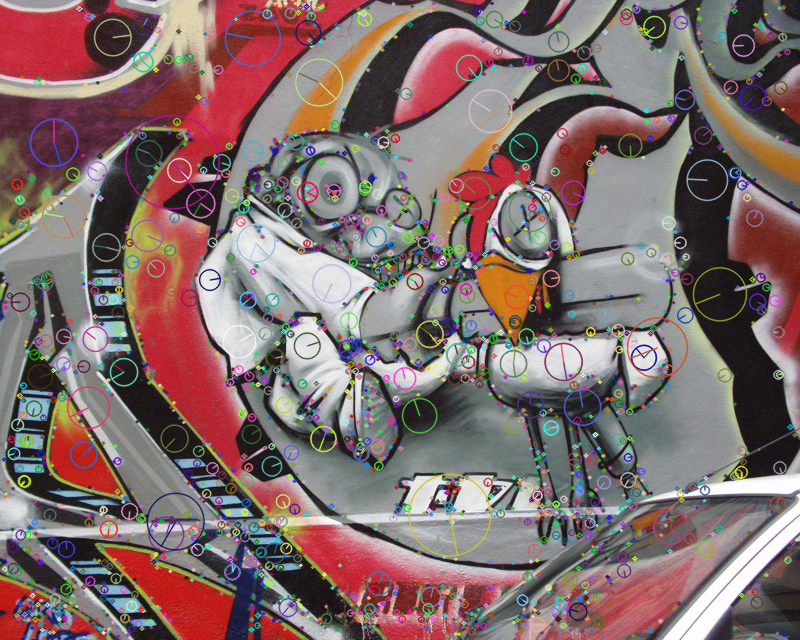
\includegraphics[width=\linewidth]{images/RobotKp}
				\label{fig:awesome_image3}
			\endminipage
			\caption{Pati}
		\end{figure}

		\begin{table}[H]
			\begin{center}
				\rowcolors{3}{}{myBlue}
				%\begin{tabular}{l | !{\vrule width -1pt}c !{\vrule width -1pt}c | !{\vrule width -1pt}c !{\vrule width -1pt}c | !{\vrule width -1pt}c !{\vrule width -1pt}c}
				\begin{tabular}{l | c c | c c | c c}
					& \multicolumn{2}{c|}{\textbf{Motos}} & \multicolumn{2}{c|}{\textbf{Barco}} & \multicolumn{2}{c}{\textbf{Ubc}} \\
					\textbf{Algorismes} & \textbf{Punts} & \textbf{Temps} & \textbf{Punts} & \textbf{Temps} & \textbf{Punts} & \textbf{Temps} \\ \hline
					Harris & 0 & 0ms & 0 & 0ms & 0 & 0ms \\
					SIFT & 0 & 0ms & 0 & 0ms & 0 & 0ms \\
					SURF & 0 & 0ms & 0 & 0ms & 0 & 0ms \\
					ORB & 0 & 0ms & 0 & 0ms & 0 & 0ms \\
					MSER & 0 & 0ms & 0 & 0ms & 0 & 0ms \\
				\end{tabular}
			\end{center}
			\caption{Detectors de keypoints - comparació}
		\end{table}
		\noindent
		També s'ha provat el sistema amb imatges reals d'entorns coneguts (la universitat i casa meva).

		\begin{figure}[!htb]
			\minipage{0.32\textwidth}
				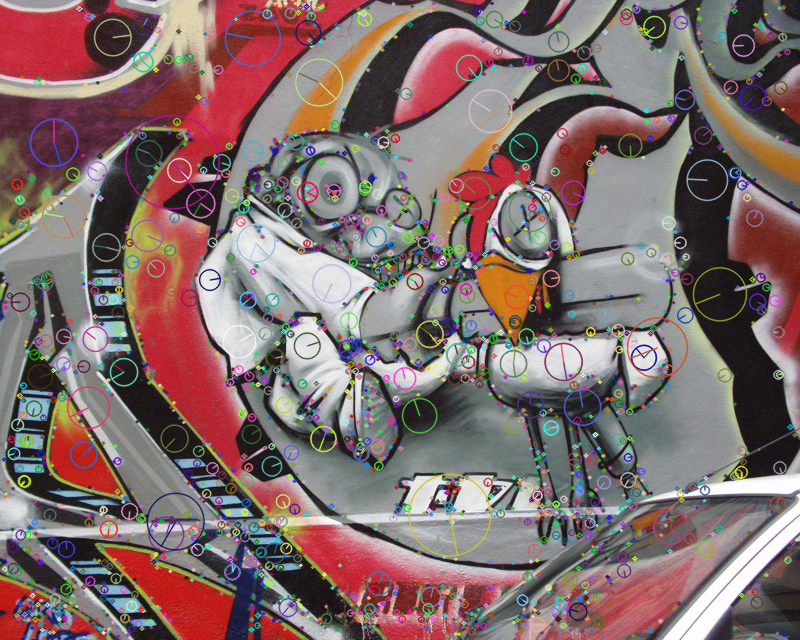
\includegraphics[width=\linewidth]{images/RobotKp}
				\label{fig:awesome_image1}
			\endminipage\hfill
			\minipage{0.32\textwidth}
				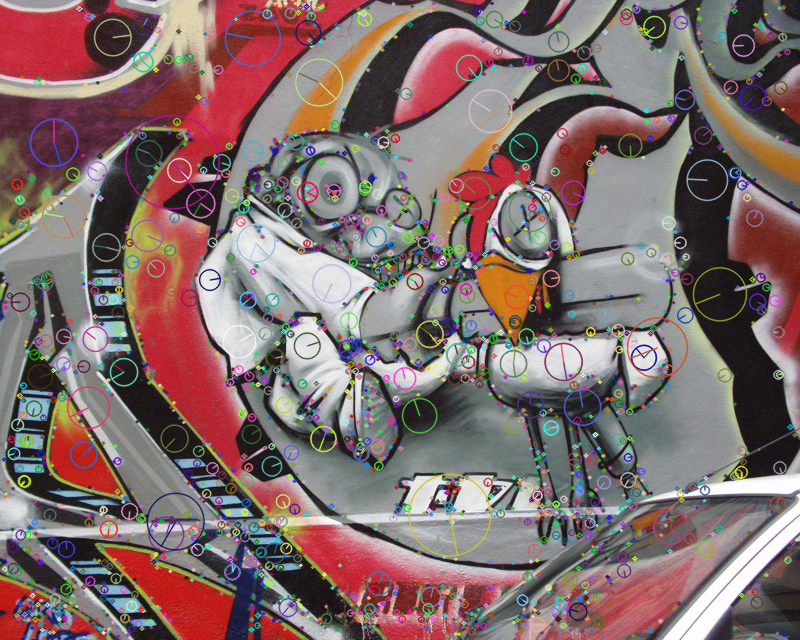
\includegraphics[width=\linewidth]{images/RobotKp}
				\label{fig:awesome_image2}
			\endminipage\hfill
			\minipage{0.32\textwidth}%
				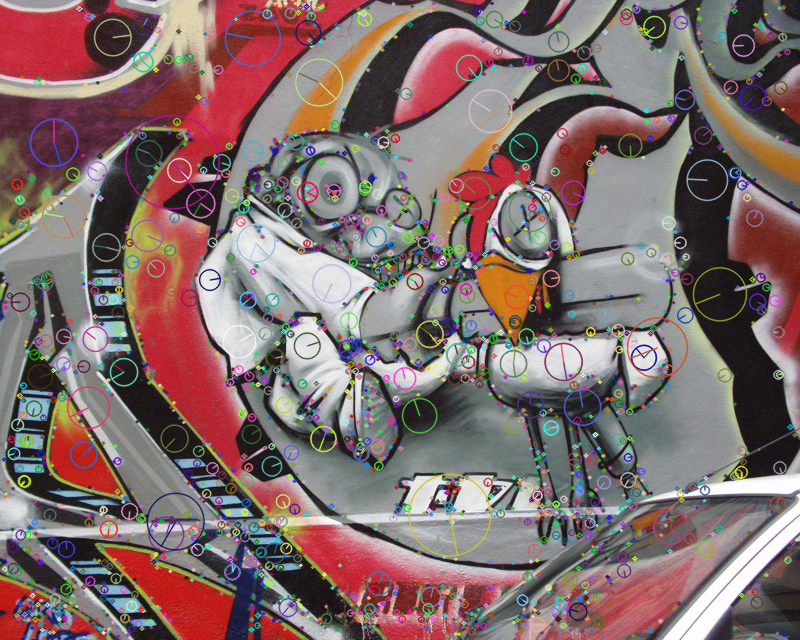
\includegraphics[width=\linewidth]{images/RobotKp}
				\label{fig:awesome_image3}
			\endminipage
			\caption{Pati}
		\end{figure}

		\begin{table}[H]
			\begin{center}
				\rowcolors{3}{}{myBlue}
				%\begin{tabular}{l | !{\vrule width -1pt}c !{\vrule width -1pt}c | !{\vrule width -1pt}c !{\vrule width -1pt}c | !{\vrule width -1pt}c !{\vrule width -1pt}c}
				\begin{tabular}{l | c c | c c | c c}
					& \multicolumn{2}{c|}{\textbf{Universitat}} & \multicolumn{2}{c|}{\textbf{Menjador}} & \multicolumn{2}{c}{\textbf{Pati}} \\
					\textbf{Algorismes} & \textbf{Punts} & \textbf{Temps} & \textbf{Punts} & \textbf{Temps} & \textbf{Punts} & \textbf{Temps} \\ \hline
					Harris & 0 & 0ms & 0 & 0ms & 0 & 0ms \\
					SIFT & 0 & 0ms & 0 & 0ms & 0 & 0ms \\
					SURF & 0 & 0ms & 0 & 0ms & 0 & 0ms \\
					ORB & 0 & 0ms & 0 & 0ms & 0 & 0ms \\
					MSER & 0 & 0ms & 0 & 0ms & 0 & 0ms \\
				\end{tabular}
			\end{center}
			\caption{Detectors de keypoints - comparació}
		\end{table}
\newpage
	\subsection{Detecció i extracció de keypoints}
		Tal com s'ha fet en l'experiment anterior, primer s'ha provat el sistema amb les imatges de visió.

		\begin{figure}[!htb]
			\minipage{0.24\textwidth}
				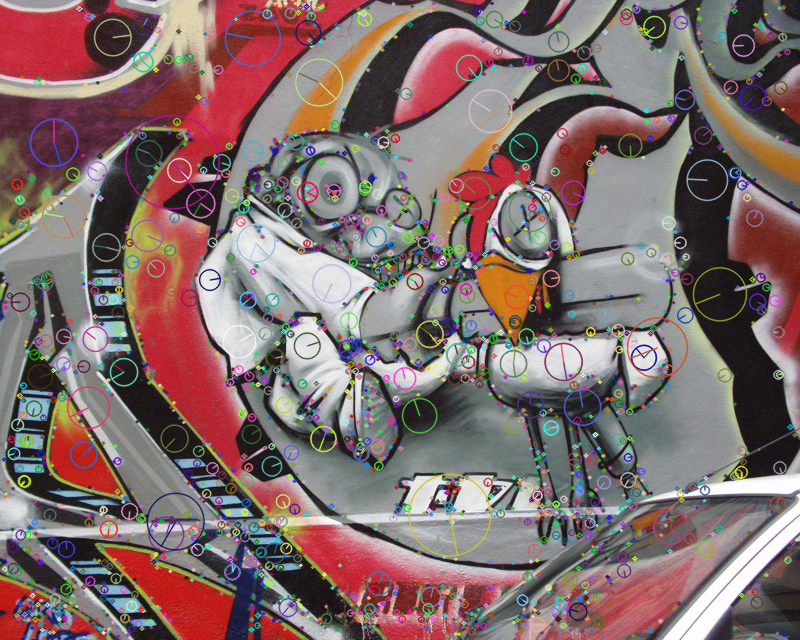
\includegraphics[width=\linewidth]{images/RobotKp}
				\label{fig:awesome_image1}
			\endminipage\hfill
			\minipage{0.24\textwidth}
				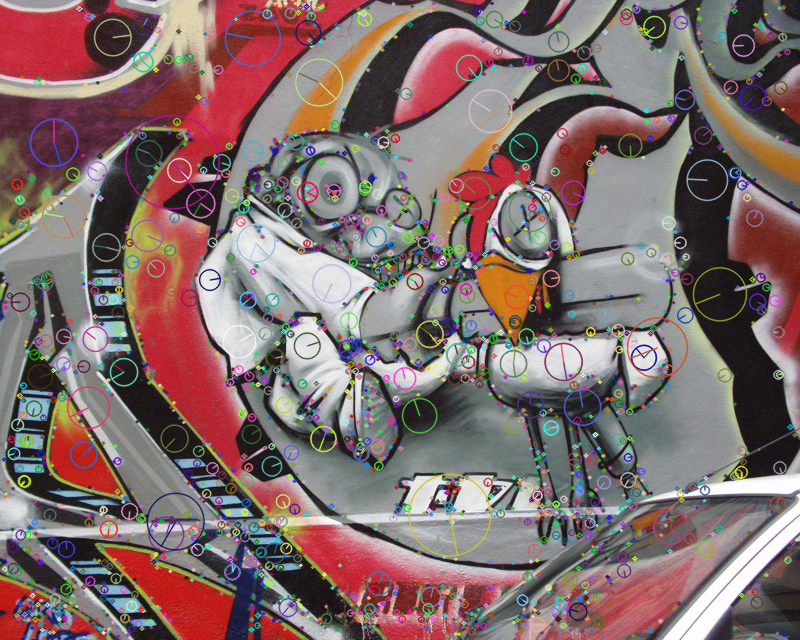
\includegraphics[width=\linewidth]{images/RobotKp}
				\label{fig:awesome_image2}
			\endminipage\hfill
			\minipage{0.24\textwidth}
				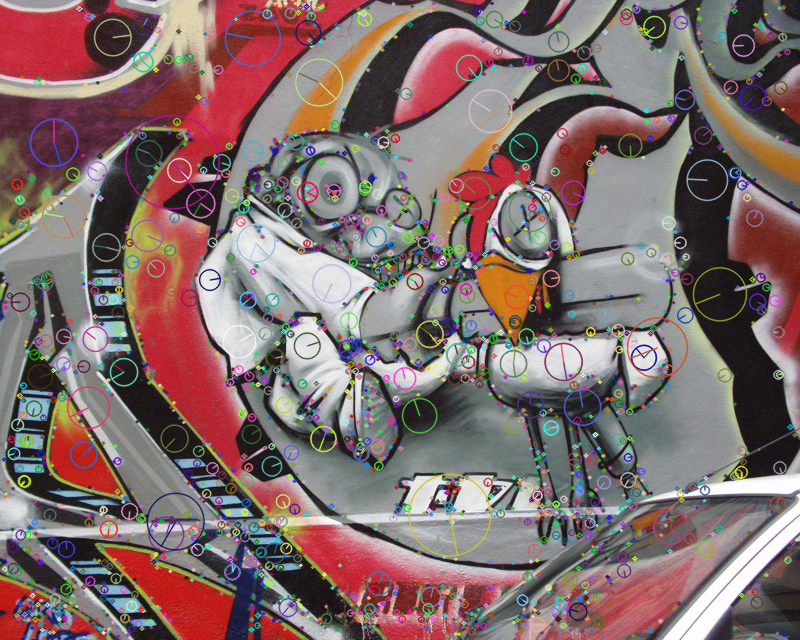
\includegraphics[width=\linewidth]{images/RobotKp}
				\label{fig:awesome_image3}
			\endminipage\hfill
			\minipage{0.24\textwidth}
				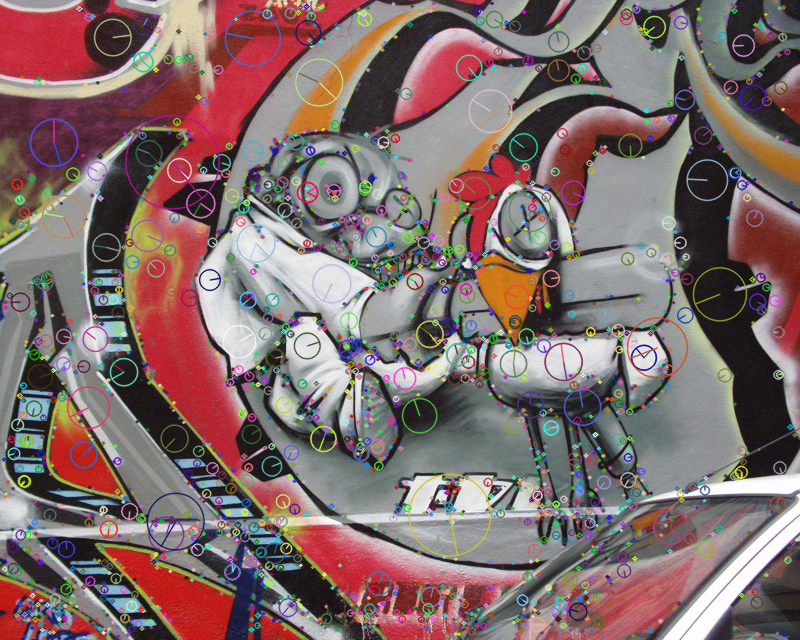
\includegraphics[width=\linewidth]{images/RobotKp}
				\label{fig:awesome_image3}
			\endminipage
			\caption{Pati}
		\end{figure}

		\begin{table}[H]
			\begin{center}
				\rowcolors{3}{}{myBlue}
				\begin{tabular}{l | c c c | c c c}
					& \multicolumn{3}{c|}{\textbf{Cotxes}} & \multicolumn{3}{c}{\textbf{Graffiti}} \\
					\textbf{Algorismes} & \textbf{Matches} & \textbf{\%} & \textbf{Temps} & \textbf{Matches} & \textbf{\%} & \textbf{Temps} \\ \hline
					Harris + SIFT & 0 & 0\% & 0ms & 0 & 0\% & 0ms \\
					Harris + LATCH & 0 & 0\% & 0ms & 0 & 0\% & 0ms \\
					SIFT + SIFT & 0 & 0\% & 0ms & 0 & 0\% & 0ms \\
					SIFT + LATCH & 0 & 0\% & 0ms & 0 & 0\% & 0ms \\
					ORB + ORB & 0 & 0\% & 0ms & 0 & 0\% & 0ms \\
					ORB + BRISK & 0 & 0\% & 0ms & 0 & 0\% & 0ms \\
					MSER + SURF & 0 & 0\% & 0ms & 0 & 0\% & 0ms \\
					MSER + DAISY & 0 & 0\% & 0ms & 0 & 0\% & 0ms \\
				\end{tabular}
			\end{center}
			\caption{Matching - comparació}
		\end{table}
		\noindent
		Les proves amb imatges reals han utilitzat les següents fotografies:

		\begin{figure}[!htb]
			\minipage{0.24\textwidth}
				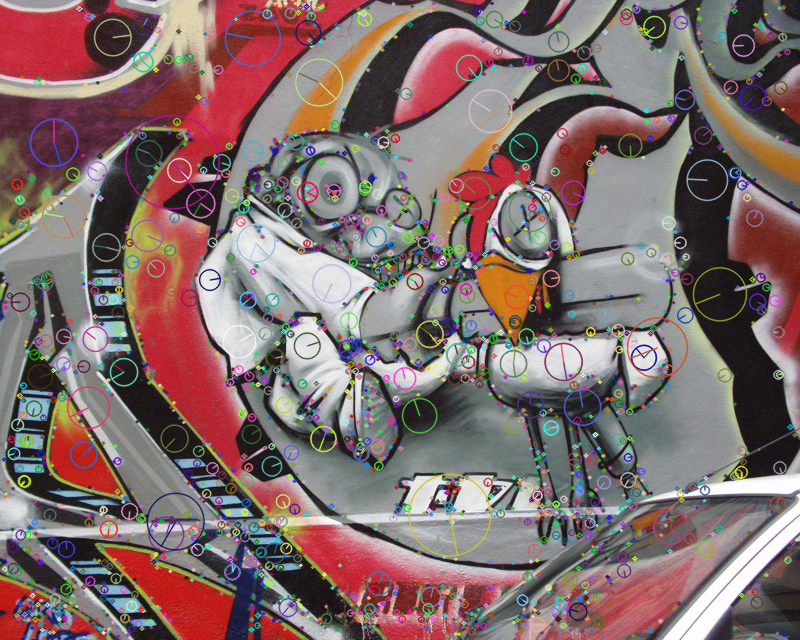
\includegraphics[width=\linewidth]{images/RobotKp}
				\label{fig:awesome_image1}
			\endminipage\hfill
			\minipage{0.24\textwidth}
				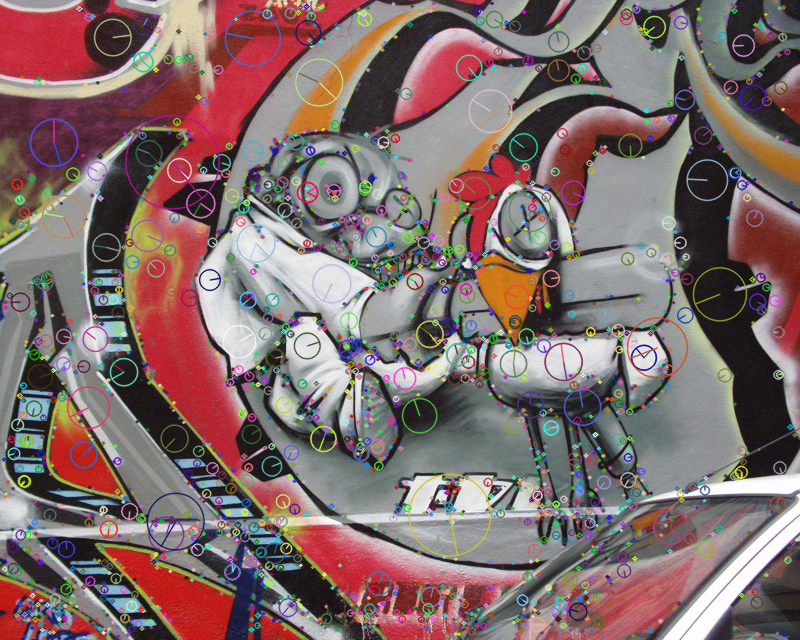
\includegraphics[width=\linewidth]{images/RobotKp}
				\label{fig:awesome_image2}
			\endminipage\hfill
			\minipage{0.24\textwidth}
				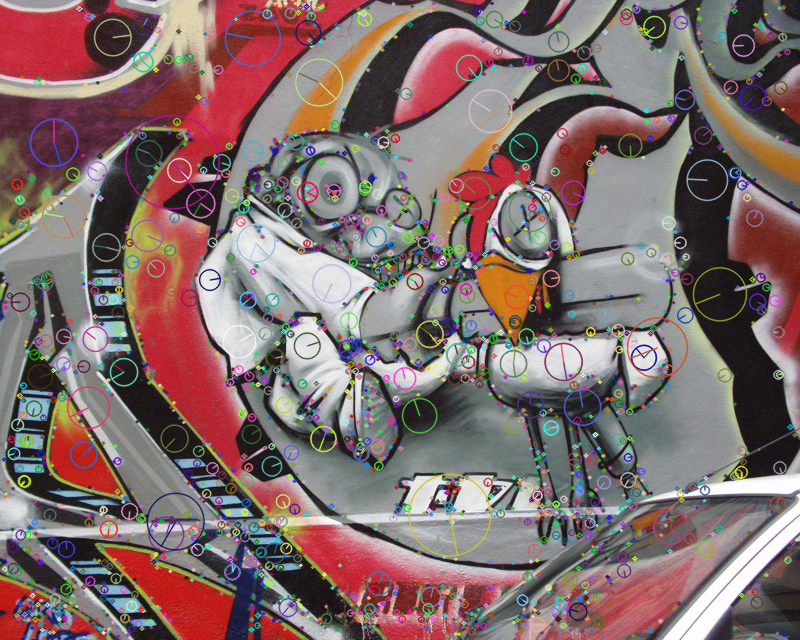
\includegraphics[width=\linewidth]{images/RobotKp}
				\label{fig:awesome_image3}
			\endminipage\hfill
			\minipage{0.24\textwidth}
				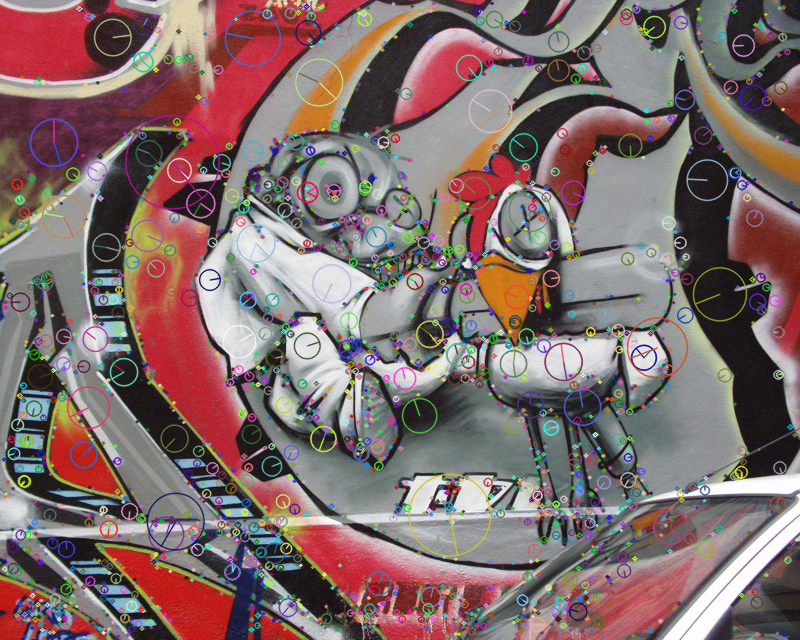
\includegraphics[width=\linewidth]{images/RobotKp}
				\label{fig:awesome_image3}
			\endminipage
			\caption{Pati}
		\end{figure}

		\begin{table}[H]
			\begin{center}
				\rowcolors{3}{}{myBlue}
				\begin{tabular}{l | c c c | c c c}
					& \multicolumn{3}{c|}{\textbf{Universitat}} & \multicolumn{3}{c}{\textbf{Menjador}} \\
					\textbf{Algorismes} & \textbf{Matches} & \textbf{\%} & \textbf{Temps} & \textbf{Matches} & \textbf{\%} & \textbf{Temps} \\ \hline
					Harris + SIFT & 0 & 0\% & 0ms & 0 & 0\% & 0ms \\
					Harris + LATCH & 0 & 0\% & 0ms & 0 & 0\% & 0ms \\
					SIFT + SIFT & 0 & 0\% & 0ms & 0 & 0\% & 0ms \\
					SIFT + LATCH & 0 & 0\% & 0ms & 0 & 0\% & 0ms \\
					ORB + ORB & 0 & 0\% & 0ms & 0 & 0\% & 0ms \\
					ORB + BRISK & 0 & 0\% & 0ms & 0 & 0\% & 0ms \\
					MSER + SURF & 0 & 0\% & 0ms & 0 & 0\% & 0ms \\
					MSER + DAISY & 0 & 0\% & 0ms & 0 & 0\% & 0ms \\
				\end{tabular}
			\end{center}
			\caption{Matching - comparació}
		\end{table}
